\documentclass[14pt]{article}

\usepackage[T2A]{fontenc}
\usepackage{amsmath}
\usepackage{graphicx}

\usepackage[utf8x]{inputenc} % Включаем поддержку UTF8  
\usepackage[russian]{babel}  % Включаем пакет для поддержки русского языка 

\graphicspath{ {./img/} }

\title{Домашнее задание на 13.02.2023}

\begin{document} \maketitle

\begin{center} №4 \end{center}

\begin{center}
    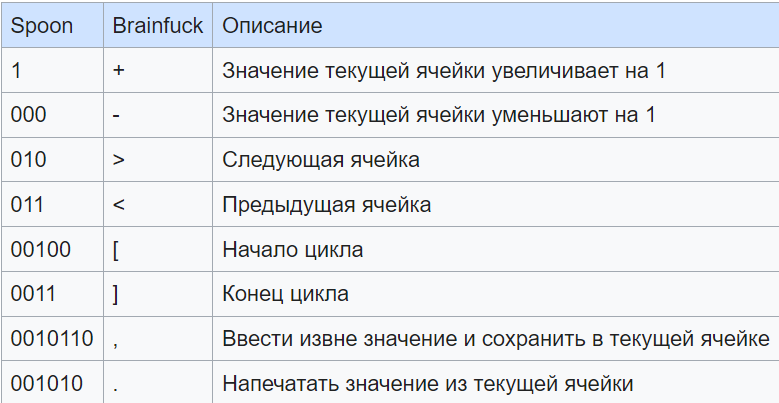
\includegraphics[scale=0.5]{scoop} \\
    
    \begin{center}
        Введем функцию $F(p, x, i)$, которая возвращает $p(x)$. \newline
        Нужна для поддержания знания о текущей ячейки $i$. \newline
        Вся программа $p$ будет обернута в $F(p, [0], 1)$ \newline
    \end{center}
    \begin{enumerate}
        \item Увеличение числа на 1 $\rightarrow N(U(x, i))$
        \item Уменьшение числа на 1 $\rightarrow dec(U(x, i)) \text{ $dec$ - где-то было в дз}$
        \item Следующая ячейка $\rightarrow$
            $$Next(x) \equiv F(p, x \cup [0], i + 1)$$
        \item Предыдущая ячейка $\rightarrow$
            $$Prev(x) \equiv F(p, x, i - 1)$$
        \item Цикл (в Scoop пока ячейка не ноль) $\rightarrow$
            $$h(x) \text{ - условие цикла}$$
            $$fc(x) \text{ - тело цикла}$$
            $$f \text{ - пустая функция}, g \text{ - $fc$ с 2-мя лишними аргументами аргументами} $$
            $$Circ \equiv R<g,f>(x, \mu(h))$$
        \item Печать $\rightarrow$ возврат результат функции
    \end{enumerate}
    
\end{center}


\end{document}
